\documentclass[14pt]{extarticle}

\usepackage[table]{xcolor} % colored lines for tables
\usepackage[normalem]{ulem} % strike through text
\usepackage{amsmath,mathtools,amsfonts,amsthm,amssymb,hyperref,pifont}
\usepackage{parskip,geometry,latexsym,bookmark,mathtools,float,cancel}
\usepackage{minted,tcolorbox,bm}

\usepackage[mathscr]{euscript}
\let\euscr\mathscr
\let\mathscr\relax
\usepackage[scr]{rsfso}
\newcommand{\ps}{\mathscr{P}} % for the Power set P

\newtheorem{defn}{Definition}
\newtheorem{thm}{Theorem}
\newtheorem{claim}{Claim}
\newtheorem{lemma}{Lemma}

\newcommand{\dps}{\displaystyle}
\newcommand{\es}{\varnothing}
\newcommand{\fbl}{\underline{\hspace{1cm}}\,\,}
\newcommand{\R}{\mathbb{R}}
\newcommand{\Q}{\mathbb{Q}}
\newcommand{\Z}{\mathbb{Z}}
\newcommand{\from}{\leftarrow}
\newcommand{\true}{{\bf t}}
\newcommand{\false}{{\bf c}}
\newcommand{\bic}{\leftrightarrow}
\newcommand{\da}{\downarrow}
\newcommand{\fa}{\forall}
\newcommand{\te}{\exists}
\newcommand{\cy}{\color{cyan}}

\newcommand{\colsq}[1]{{\color{#1} $\blacksquare$}}

\newcommand{\base}[1]{{\cy #1}} % for log bases
\newcommand{\floor}[1]{{\left\lfloor#1\right\rfloor}}
\newcommand{\ceil}[1]{{\left\lceil#1\right\rceil}}
\newcommand\Ccancel[2][black]{\renewcommand\CancelColor{\color{#1}}\cancel{#2}}
\newcommand\Cbcancel[2][black]{\renewcommand\CancelColor{\color{#1}}\bcancel{#2}}

\renewcommand{\arraystretch}{1.2}

\hypersetup{colorlinks,allcolors=blue,linktoc=all}
\geometry{a4paper}
\geometry{margin=0.42in}

\title{Solutions to Chapter 7, Susanna Epp Discrete Math 5th Edition}

\author{https://github.com/spamegg1}

\begin{document}
\maketitle
\tableofcontents

\section{Exercise Set 7.1}

\subsection{Exercise 1}
Let \(X = \{1, 3, 5\}\) and \(Y = \{s, t, u, v\}\). Define \(f: X \to Y\) by the following arrow diagram.

\begin{figure}[ht!]
\centering
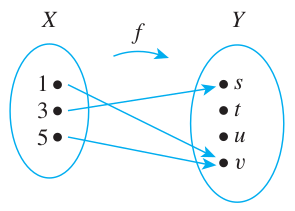
\includegraphics[scale=0.5]{../images/7.1.1.png}
\end{figure}

\subsubsection{(a)}
Write the domain of $f$ and the co-domain of $f$.

\begin{proof}
domain of \(f = \{1, 3, 5\}\), co-domain of \(f = \{s, t, u, v\}\)
\end{proof}

\subsubsection{(b)}
Find $f(1), f(3)$, and $f(5)$.

\begin{proof}
\(f(1) = v, f(3) = s, f(5) = v\)
\end{proof}

\subsubsection{(c)}
What is the range of $f$?

\begin{proof}
range of \(f = \{s, v\}\)
\end{proof}

\subsubsection{(d)}
Is 3 an inverse image of $s$? Is 1 an inverse image of $u$?

\begin{proof}
yes, no
\end{proof}

\subsubsection{(e)}
What is the inverse image of $s$? of $u$? of $v$?

\begin{proof}
inverse image of \(s = \{3\}\), inverse image of \(u = \es\), inverse image of \(v = \{1, 5\}\)
\end{proof}

\subsubsection{(f)}
Represent $f$ as a set of ordered pairs.

\begin{proof}
\(\{(1, v), (3, s), (5, v)\}\)
\end{proof}

\subsection{Exercise 2}
Let \(X = \{1, 3, 5\}\) and \(Y = \{a, b, c, d\}\). Define \(g: X \to Y\) by the following arrow diagram.

\begin{figure}[ht!]
\centering
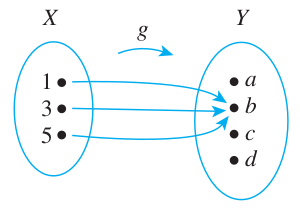
\includegraphics[scale=0.6]{../images/7.1.2.png}
\end{figure}

\subsubsection{(a)}
Write the domain of $g$ and the co-domain of $g$.

\begin{proof}
domain: \(\{1, 3, 5\}\) co-domain: \(\{a,b,c,d\}\)
\end{proof}

\subsubsection{(b)}
Find $g(1), g(3)$, and $g(5)$.

\begin{proof}
\(g(1) = b, g(3) = b, g(5) = b\)
\end{proof}

\subsubsection{(c)}
What is the range of $g$?

\begin{proof}
\(\{b\}\)
\end{proof}

\subsubsection{(d)}
Is 3 an inverse image of $a$? Is 1 an inverse image of $b$?

\begin{proof}
no, yes
\end{proof}

\subsubsection{(e)}
What is the inverse image of $b$? of $c$?

\begin{proof}
\(\{1,3,5\}\) and $\es$
\end{proof}

\subsubsection{(f)}
Represent $g$ as a set of ordered pairs.

\begin{proof}
\(\{(1,b),(3,b),(5,b)\}\)
\end{proof}


\subsection{Exercise 3}
Indicate whether the statements in parts (a)–(d) are true or false for all functions. Justify your answers.

\subsubsection{(a)}
If two elements in the domain of a function are equal, then their images in the co-domain are equal.

\begin{proof}
True. The definition of function says that for any input there is one and only one output, so if two inputs are 
equal, their outputs must also be equal.
\end{proof}

\subsubsection{(b)}
If two elements in the co-domain of a function are equal, then their preimages in the domain are also equal.

\begin{proof}
Not necessarily true. A function can have the same output for more than one input.
\end{proof}

\subsubsection{(c)}
A function can have the same output for more than one input.

\begin{proof}
True. The definition of function does not prohibit this occurrence.
\end{proof}

\subsubsection{(d)}
A function can have the same input for more than one output.

\begin{proof}
False, this is ruled out by the definition of a function. Functions are single valued. Every input corresponds to 
only one output.
\end{proof}

\subsection{Exercise 4}
\subsubsection{(a)}
Find all functions from \(X = \{a, b\}\) to \(Y = \{u, v\}\).

\begin{proof}
There are four functions from $X$ to $Y$ as shown {\it on the next page}.

\begin{figure}[ht!]
\centering
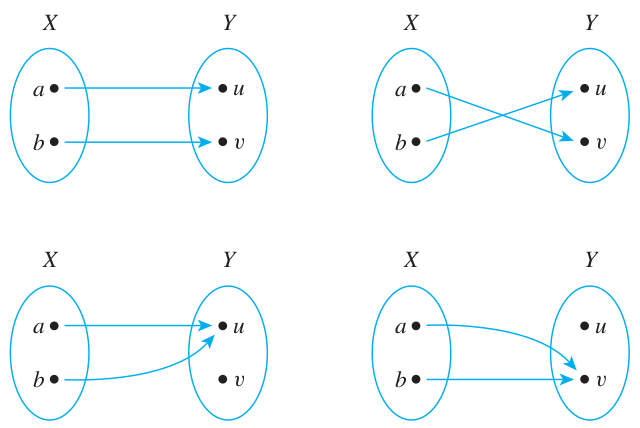
\includegraphics[scale=0.5]{../images/7.1.4.a.png}
\end{figure}

\end{proof}

\subsubsection{(b)}
Find all functions from \(X = \{a, b, c\}\) to \(Y = \{u\}\).

\begin{proof}
There is only one function $f: X \to Y$ given by the set \(\{(a,u), (b,u), (c,u)\}\).
\end{proof}

\subsubsection{(c)}
Find all functions from \(X = \{a, b, c\}\) to \(Y = \{u, v\}\).

\begin{proof}
There are 8 functions:

\(\{(a,u), (b,u), (c,u)\}\)

\(\{(a,u), (b,u), (c,v)\}\)

\(\{(a,u), (b,v), (c,u)\}\)

\(\{(a,u), (b,v), (c,v)\}\)

\(\{(a,v), (b,u), (c,u)\}\)

\(\{(a,v), (b,u), (c,v)\}\)

\(\{(a,v), (b,v), (c,u)\}\)

\(\{(a,v), (b,v), (c,v)\}\)
\end{proof}

\subsection{Exercise 5}
Let $I_{\Z}$ be the identity function defined on the set of all integers, and suppose that \(e, b_{i}^{jk}, K(t)\), and 
\(u_{kj}\) all represent integers. Find the following:

\subsubsection{(a)}
\(I_{\Z}(e)\)

\begin{proof}
$e$ (because \(I_{\Z}\) is the identity function).
\end{proof}

\subsubsection{(b)}
\(I_{\Z}(b_{i}^{jk})\)

\begin{proof}
$b_{i}^{jk}$ (because \(I_{\Z}\) is the identity function).
\end{proof}

\subsubsection{(c)}
\(I_{\Z}(K(t))\)

\begin{proof}
$K(t)$ (because \(I_{\Z}\) is the identity function).
\end{proof}

\subsubsection{(d)}
\(I_{\Z}(u_{kj})\)

\begin{proof}
$u_{kj}$ (because \(I_{\Z}\) is the identity function).
\end{proof}

\subsection{Exercise 6}
Find functions defined on the set of nonnegative integers that can be used to define the sequences whose first six 
terms are given below.

\subsubsection{(a)}
\(\dps 1, -\frac{1}{3}, \frac{1}{5}, -\frac{1}{7}, \frac{1}{9}, -\frac{1}{11}\)

\begin{proof}
The sequence is given by the function \(f: \Z^{nonneg} \to \R\) defined by the rule \(\dps f(n)=\frac{(-1)^n}{2n+1}\)
{\cy for each nonnegative integer $n$.}
\end{proof}

\subsubsection{(b)}
\(0, -2, 4, -6, 8, -10\)

\begin{proof}
The sequence is given by the function \(f: \Z^{nonneg} \to \Z\) defined by the rule \(\dps f(n) = (-1)^n \cdot (2n)\)
{\cy for each nonnegative integer $n$.}
\end{proof}

\subsection{Exercise 7}
Let \(A = \{1, 2, 3, 4, 5\}\), and define a function \(F: \ps(A) \to \Z\) as follows: For each set $X$ in $\ps(A)$,
\[
F(x) =
\left\{
\begin{tabular}{ll}
\(0\) & if $X$ has an even number of elements \\
\(1\) & if $X$ has an odd number of elements
\end{tabular}
\right.
\]
Find the following:

\subsubsection{(a)}
\(F(\{1, 3, 4\})\) 

\begin{proof}
\(F(\{1, 3, 4\}) = 1\) {\it [because \(\{1, 3, 4\}\) has an odd number of elements]}

\end{proof}

\subsubsection{(b)}
\(F(\es)\)

\begin{proof}
\(F(\{\es\}) = 0\) {\it [because \(\{\es\}\) has an even number of elements]}
\end{proof}

\subsubsection{(c)}
\(F(\{2, 3\})\)

\begin{proof}
\(F(\{2, 3\}) = 0\) {\it [because \(\{2, 3\}\) has an even number of elements]}
\end{proof}

\subsubsection{(d)}
\(F(\{2, 3, 4, 5\})\)

\begin{proof}
\(F(\{2, 3, 4, 5\}) = 0\) {\it [because \(\{2, 3, 4, 5\}\) has an even number of elements]}
\end{proof}

\subsection{Exercise 8}
Let \(J_5 = \{0, 1, 2, 3, 4\}\), and define a function \(F: J_5 \to J_5\) as follows: For each \(x \in J_5, F(x) = (x^3 
+ 2x + 4) \mod 5\). Find the following:

\subsubsection{(a)}
$F(0)$

\begin{proof}
\(F(0) = (0^3 + 2 \cdot 0 + 4) \mod 5 = 4 \mod 5 = 4\)

\end{proof}

\subsubsection{(b)}
$F(1)$

\begin{proof}
\(F(1) = (1^3 + 2 \cdot 1 + 4) \mod 5 = 7 \mod 5 = 2\)
\end{proof}

\subsubsection{(c)}
$F(2)$

\begin{proof}
\(F(2) = (2^3 + 2 \cdot 2 + 4) \mod 5 = 16 \mod 5 = 1\)
\end{proof}

\subsubsection{(d)}
$F(3)$

\begin{proof}
\(F(3) = (3^3 + 2 \cdot 3 + 4) \mod 5 = 37 \mod 5 = 2\)
\end{proof}

\subsubsection{(e)}
$F(4)$

\begin{proof}
\(F(4) = (4^3 + 2 \cdot 4 + 4) \mod 5 = 76 \mod 5 = 1\)
\end{proof}

\subsection{Exercise 9}
Define a function \(S: \Z^+ \to \Z^+\) as follows: For each positive integer \(n, S(n) =\) the sum of the positive 
divisors of $n$. Find the following:

\subsubsection{(a)}
$S(1)$

\begin{proof}
$S(1) = 1$

\end{proof}

\subsubsection{(b)}
$S(15)$

\begin{proof}
\(S(15) = 1 + 3 + 5 + 15 = 24\)
\end{proof}

\subsubsection{(c)}
$S(17)$

\begin{proof}
\(S(15) = 1 + 17 = 18\)
\end{proof}

\subsubsection{(d)}
$S(5)$

\begin{proof}
\(S(5) = 1 + 5 = 6\)
\end{proof}

\subsubsection{(e)}
$S(18)$

\begin{proof}
\(S(18) = 1 + 2 + 3 + 6 + 9 + 18 = 39\)
\end{proof}

\subsubsection{(f)}
$S(21)$

\begin{proof}
\(S(21) = 1 + 3 + 7 + 21 = 32\)
\end{proof}

\subsection{Exercise 10}
Let $D$ be the set of all finite subsets of positive integers. Define a function \(T: \Z^+ \to D\) as follows: 
For each positive integer \(n, T(n) =\) the set of positive divisors of $n$. Find the following:

\subsubsection{(a)}
$T(1)$

\begin{proof}
\(T(1) = \{1\}\)

\end{proof}

\subsubsection{(b)}
$T(15)$

\begin{proof}
\(T(15) = \{1, 3, 5, 15\}\)
\end{proof}

\subsubsection{(c)}
$T(17)$

\begin{proof}
\(T(17) = \{1, 17\}\)
\end{proof}

\subsubsection{(d)}
$T(5)$

\begin{proof}
\(T(1) = \{1\}\)
\end{proof}

\subsubsection{(e)}
$T(18)$

\begin{proof}
\(T(18) = \{1, 2, 3, 6, 9, 18\}\)
\end{proof}

\subsubsection{(f)}
$T(21)$

\begin{proof}
\(T(21) = \{1, 3, 7, 21\}\)
\end{proof}

\subsection{Exercise 11}
Define \(F: \Z \times \Z \to \Z \times \Z\) as follows: For every ordered pair \((a,b)\) of integers, \(F(a,b) = (2a+1, 
3b-2)\). Find the following:

\subsubsection{(a)}
$F(4,4)$

\begin{proof}
\(F(4, 4) = (2 \cdot 4 + 1, 3 \cdot 4 - 2) = (9, 10)\)
\end{proof}

\subsubsection{(b)}
$F(2,1)$

\begin{proof}
\(F(2, 1) = (2 \cdot 2 + 1, 3 \cdot 1 - 2) = (5, 1)\)
\end{proof}

\subsubsection{(c)}
$F(3,2)$

\begin{proof}
\(F(3, 3) = (2 \cdot 3 + 1, 3 \cdot 3 - 2) = (7, 7)\)
\end{proof}

\subsubsection{(d)}
$F(1,5)$

\begin{proof}
\(F(1, 5) = (2 \cdot 1 + 1, 3 \cdot 5 - 2) = (3, 13)\)
\end{proof}

\subsection{Exercise 12}
Let \(J_5 = \{0, 1, 2, 3, 4\}\), and define \(G: J_5 \times J_5 \to J_5 \times J_5\) as follows: For each \((a,b) \in 
J_5 \times J_5, G(a,b) = ((2a+1) \mod 5, (3b-2) \mod 5)\). Find the following:

\subsubsection{(a)}
$G(4,4)$

\begin{proof}
\(G(4, 4) = ((2 \cdot 4 + 1) \mod 5, (3 \cdot 4 - 2) \mod 5) = (9 \mod 5, 10 \mod 5) = (4, 0)\)
\end{proof}

\subsubsection{(b)}
$G(2,1)$

\begin{proof}
\(G(2, 1) = ((2 \cdot 2 + 1) \mod 5, (3 \cdot 1 - 2) \mod 5) = (5 \mod 5, 1 \mod 5) = (0, 1)\)
\end{proof}

\subsubsection{(c)}
$G(3,2)$

\begin{proof}
\(G(3, 2) = ((2 \cdot 3 + 1) \mod 5, (3 \cdot 2 - 2) \mod 5) = (7 \mod 5, 4 \mod 5) = (2, 4)\)
\end{proof}

\subsubsection{(d)}
$G(1,5)$

\begin{proof}
\(G(1, 5) = ((2 \cdot 1 + 1) \mod 5, (3 \cdot 5 - 2) \mod 5) = (3 \mod 5, 13 \mod 5) = (3, 3)\)
\end{proof}

\subsection{Exercise 13}
Let \(J_5 = \{0, 1, 2, 3, 4\}\), and define functions \(f: J_5 \to J_5\) and \(g: J_5 \to J_5\) as follows: For each 
\(x \in J_5, f(x) = (x + 4)^2 \mod 5\) and \(g(x) = (x^2 + 3x + 1) \mod 5\). Is $f = g$? Explain.

\begin{proof}
\begin{center}
\arrayrulecolor{cyan}
\begin{tabular}{|c|c|c|}
\hline
$x$ & $f(x)$ & $g(x)$ \\
\hline
0 & \(4^2 \mod 5 = 1\) & \((0^2 + 3 \cdot 0 + 1) \mod 5 = 1\) \\
\hline
1 & \(5^2 \mod 5 = 0\) & \((1^2 + 3 \cdot 1 + 1) \mod 5 = 0\) \\
\hline
2 & \(6^2 \mod 5 = 1\) & \((2^2 + 3 \cdot 2 + 1) \mod 5 = 1\) \\
\hline
3 & \(7^2 \mod 5 = 4\) & \((3^2 + 3 \cdot 3 + 1) \mod 5 = 4\) \\
\hline
4 & \(8^2 \mod 5 = 4\) & \((4^2 + 3 \cdot 4 + 1) \mod 5 = 4\) \\
\hline
\end{tabular}
\arrayrulecolor{black}
\end{center}

The table shows that \(f(x) = g(x)\) for every $x$ in \(J_5\). Thus, by definition of equality of functions, $f = g$.
\end{proof}

\subsection{Exercise 14}
Define functions $H$ and $K$ from $\R$ to $\R$ by the following formulas: For every \(x \in \R, H(x) = \floor{x} 
+ 1\) and \(K(x) = \ceil{x}\). Does $H = K$? Explain.

\begin{proof}
No, because \(H(2) = \floor{2} + 1 = 3 \neq 2 = \ceil{2} = K(2)\).
\end{proof}

\subsection{Exercise 15}
Let $F$ and $G$ be functions from the set of all real numbers to itself. Define new functions 
\(F \cdot G: \R \to \R\) and \(G \cdot F: \R \to \R\) as follows: For every \(x \in \R\), 
\((F \cdot G)(x) = F(x) \cdot G(x)\), \((G \cdot F)(x) = G(x) \cdot F(x)\). Does $F \cdot G = G \cdot F$? Explain.

\begin{proof}
\begin{tabular}{rcll}
\((F \cdot G)(x)\) & = & \(F(x) \cdot G(x)\) & {\cy by definition of $F \cdot G$} \\
& = & \(G(x) \cdot F(x)\) & {\cy by commutative law for real numbers} \\
& = & \((G \cdot F)(x)\) & {\cy by definition of $G \cdot F$}
\end{tabular}

for every real number $x$. Therefore $F\cdot G$ and $G \cdot F$ are equal.
\end{proof}

\subsection{Exercise 16}
Let $F$ and $G$ be functions from the set of all real numbers to itself. Define new functions 
\(F - G: \R \to \R\) and \(G - F: \R \to \R\) as follows: For every \(x \in \R\), \((F - G)(x) = F(x) - G(x)\), 
\((G - F)(x) = G(x) - F(x)\). Does $F - G = G - F$? Explain.

\begin{proof}
\underline{Counterexample:} Let \(F(x) = 2x, G(x) = 3x\). 
Then 
\[
(F-G)(1) = F(1) - G(1) = 2 - 3 = -1 \neq 1 = 3 - 2 = G(1) - F(1) = (G-F)(1).
\] 
Therefore $F - G$ does not equal $G - F$.
\end{proof}

\subsection{Exercise 17}
Use the definition of logarithm to fill in the blanks below.

\subsubsection{(a)}
\(\log_{2} 8 = 3\) because \fbl.

\begin{proof}
\(2^3 = 8\)
\end{proof}

\subsubsection{(b)}
\(\log_{5}(\frac{1}{25}) = -2\) because \fbl.

\begin{proof}
\(\dps 5^{-2} = \frac{1}{25}\)
\end{proof}

\subsubsection{(c)}
\(\log_{4} 4 = 1\) because \fbl.

\begin{proof}
\(4^1 = 4\)
\end{proof}

\subsubsection{(d)}
\(\log_{3}(3^n) = n\) because \fbl.

\begin{proof}
\(3^n = 3^n\)
\end{proof}

\subsubsection{(e)}
\(\log_{4} 1 = 0\) because \fbl.

\begin{proof}
\(4^0 = 1\)
\end{proof}

\subsection{Exercise 18}
Find exact values for each of the following quantities without using a calculator.

\subsubsection{(a)}
\(\log_{3} 81\)

\begin{proof}
4
\end{proof}

\subsubsection{(b)}
\(\log_{2} 1024\)

\begin{proof}
10
\end{proof}

\subsubsection{(c)}
\(\log_{3} \frac{1}{27}\)

\begin{proof}
$-3$
\end{proof}

\subsubsection{(d)}
\(\log_{2} 1\)

\begin{proof}
0
\end{proof}

\subsubsection{(e)}
\(\log_{10}(\frac{1}{10})\)

\begin{proof}
$-1$
\end{proof}

\subsubsection{(f)}
\(\log_{3} 3\)

\begin{proof}
1
\end{proof}

\subsubsection{(g)}
\(\log_{2} 2^k\)

\begin{proof}
$k$
\end{proof}

\subsection{Exercise 19}
Use the definition of logarithm to prove that for any positive real number $b$ with \(b \neq 1, \log_b b = 1\).

\begin{proof}
Let $b$ be any positive real number with \(b \neq 1\). Since \(b^1 = b\), then \(\log_b b = 1\) by definition of logarithm.
\end{proof}

\subsection{Exercise 20}
Use the definition of logarithm to prove that for any positive real number $b$ with \(b \neq 1, \log_b 1 = 0\).

\begin{proof}
Let $b$ be any positive real number with \(b \neq 1\). Since \(b^0 = 1\), then \(\log_b 1 = 0\) by definition of logarithm.
\end{proof}

\subsection{Exercise 21}
If $b$ is any positive real number with \(b \neq 1\) and $x$ is any real number, \(b^{-x}\) is defined as follows: 
\(\dps b^{-x} = \frac{1}{b^x}\). Use this definition and the definition of logarithm to prove that \(\dps \log_b 
\left(\frac{1}{u}\right) = -\log_b(u)\) for all positive real numbers $u$ and $b$, with \(b \neq 1\).

\begin{proof}
Suppose $b$ and $u$ are any positive real numbers with \(b \neq 1\). {\it [We must show that \(\log_b (\frac{1}{u}) = 
-\log_b(u)\).]} Let \(v = \log_b (\frac{1}{u})\). By definition of logarithm, \(b^v = \frac{1}{u}\). Multiplying 
both sides by $u$ and dividing by $b^v$ gives \(u=b^{-v}\), and thus, by definition of logarithm, \(-v = \log_b(u)\). 
When both sides of this equation are multiplied by $-1$, the result is \(v = -\log_b(u)\). Therefore, \(\log_b 
(\frac{1}{u}) = - \log_b(u)\) because both expressions equal $v$. {\it [This is what was to be shown.]}
\end{proof}

\subsection{Exercise 22}
Use the unique factorization for the integers theorem (Section 4.4) and the definition of logarithm to prove that 
$\log_3(7)$ is irrational.

\begin{proof}
1. Argue by contradiction and assume \(r = \log_3(7)\) is rational.

2. By 1 and definition of rational, \(r = a / b\) for some integers $a,b$ where $b \neq 0$.

3. We may assume \(b > 0\). (If \(b < 0\) then \(a/b = (-a)/(-b)\) therefore we can replace $a/b$ with $-a/(-b)$
where \(-b > 0\).)

4. By 1, 2 and definition of logarithm, \(7 = 3^{a/b}\).

5. By 4, taking the $b$th powers of both sides, we get \(7^b = 3^a\).

6. Since \(b\) is a positive integer, \(7^b\) is a positive integer. Therefore \(3^a\) is the same positive integer.

7. By 6, we have two different prime factorizations of the same positive integer. By the uniqueness part of the prime
factorization theorem, this is only possible if the positive integer is equal to 1.

8. By 7, \(7^b = 3^a = 1\) so \(a = b = 0\). This is a contradiction since \(b > 0\).

9. So our supposition in 1 is false by 8, thus \(\log_3(7)\) is irrational.
\end{proof}

\subsection{Exercise 23}
If $b$ and $y$ are positive real numbers such that \(\log_b y = 3\), what is \(\log_{1/b}(y)\)? Explain.

\begin{proof}
By definition of logarithm with base $b$, \(b^3 = y\). So
\[
y = b^3 = \frac{1}{\frac{1}{b^3}} = \frac{1}{\left(\frac{1}{b}\right)^3} = \left(\frac{1}{b}\right)^{-3}
\]
So by definition of logarithm with base $1/b$, \(\log_{1/b}(y) = -3\).
\end{proof}

\subsection{Exercise 24}
If $b$ and $y$ are positive real numbers such that \(\log_b y = 2\), what is \(\log_{b^2}(y)\)? Explain.

\begin{proof}
By definition of logarithm with base $b$, \(b^2 = y\). So
by definition of logarithm with base $b^2$, 
\(\log_{b^2}(y) = 1\) because \((b^2)^1 = y\).
\end{proof}

\subsection{Exercise 25}
Let \(A = \{2, 3, 5\}\) and \(B = \{x, y\}\). Let $p_1$ and $p_2$ be the projections of \(A \times B\) onto the first 
and second coordinates. That is, for each pair \((a, b) \in A \times B, p_1(a, b) = a\) and \(p_2(a, b) = b\).

\subsubsection{(a)}
Find \(p_1(2, y)\) and \(p_1(5, x)\). What is the range of $p_1$?

\begin{proof}
\(p_1(2, y) = 2, p_1(5, x) = 5\), range of \(p_1 = \{2, 3, 5\}\)
\end{proof}

\subsubsection{(b)}
Find \(p_2(2, y)\) and \(p_2(5, x)\). What is the range of $p_2$?

\begin{proof}
\(p_2(2, y) = y, p_2(5, x) = x\), range of \(p_2 = \{x, y\}\)
\end{proof}

\subsection{Exercise 26}
Observe that mod and div can be defined as functions from \(\Z^{nonneg} \times \Z^+\) to $\Z$. For each ordered pair 
\((n, d)\) consisting of a nonnegative integer $n$ and a positive integer $d$, let

\(mod(n, d) = n \mod d\) (the nonnegative remainder obtained when $n$ is divided by $d$).

\(div(n, d) = n \text{ div } d\) (the integer quotient obtained when $n$ is divided by $d$).

Find each of the following:

\subsubsection{(a)}
\(mod(67, 10)\) and \(div(67, 10)\)

\begin{proof}
\(mod(67, 10) = , div(67, 10) = \)
\end{proof}

\subsubsection{(b)}
$mod(59, 8)$ and $div(59, 8)$

\begin{proof}
\(mod(67, 10) = 7, div(67, 10) = 6\)
\end{proof}

\subsubsection{(c)}
$mod(30, 5)$ and $div(30, 5)$

\begin{proof}
\(mod(30, 5) = 0, div(30, 5) = 6\)
\end{proof}

\subsection{Exercise 27}
Let $S$ be the set of all strings of $a$’s and $b$’s.

\subsubsection{(a)}
Define \(f: S \to \Z\) as follows: For each string $s$ in $S$
\[
f(s) =
\left\{
\begin{tabular}{lr}
the number of $b$'s to the left of the left most $a$ in $s$ & if $s$ contains some $a$'s \\
0 & if $s$ contains no $a$'s
\end{tabular}
\right.
\]
Find \(f(aba), f(bbab)\), and \(f(b)\). What is the range of $f$?

\begin{proof}
\(f(aba) = 0\) {\it [because there are no $b$'s to the left
of the leftmost $a$ in $aba$]}

\(f(bbab) = 2\) {\it [because there are two $b$'s to the left of the leftmost $a$ in $bbab$]}

\(f(b) = 0\) {\it [because the string $b$ contains no $a$'s]}

range of \(f = \Z^{nonneg}\)
\end{proof}

\subsubsection{(b)}
Define \(g: S \to S\) as follows: For each string $s$ in $S$, \(g(s) =\) the string obtained by writing the 
characters of $s$ in reverse order. Find \(g(aba), g(bbab)\), and \(g(b)\). What is the range of $g$?

\begin{proof}
\(g(aba) = aba, g(bbab) = babb, g(b) = b\), range of \(g = S\)
\end{proof}

\subsection{Exercise 28}
Consider the coding and decoding functions $E$ and $D$ defined in Example 7.1.9.

\subsubsection{(a)}
Find \(E(0110)\) and \(D(111111000111)\).

\begin{proof}
\(E(0110) = 000111111000\) and \(D(111111000111) = 1101\)
\end{proof}

\subsubsection{(b)}
Find \(E(1010)\) and \(D(000000111111)\).

\begin{proof}
\(E(1010) = 111000111000\) and \(D(000000111111) = 0011\)
\end{proof}

\subsection{Exercise 29}
Consider the Hamming distance function defined in Example 7.1.10.

\subsubsection{(a)}
Find \(H(10101, 00011)\).

\begin{proof}
\(H(10101, 00011)\) = 3
\end{proof}

\subsubsection{(b)}
Find \(H(00110, 10111)\).

\begin{proof}
\(H(00110, 10111)\) = 2
\end{proof}

\subsection{Exercise 30}
Draw arrow diagrams for the Boolean functions defined by the following input/output tables.

\subsubsection{(a)}
\begin{center}
\arrayrulecolor{cyan}
\begin{tabular}{|cc|c|}
\hline
\multicolumn{2}{|c|}{\cy Input} & {\cy Output} \\
\hline
$P$ & $Q$ & $R$ \\
\hline
1 & 1 & 0 \\
\hline
1 & 0 & 1 \\
\hline
0 & 1 & 0 \\
\hline
0 & 0 & 1 \\
\hline
\end{tabular}
\arrayrulecolor{black}
\end{center}

\begin{proof}
\begin{figure}[ht!]
\centering
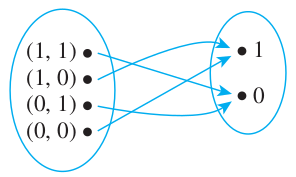
\includegraphics[scale=0.6]{../images/7.1.30.a.png}
\end{figure}
\end{proof}

\subsubsection{(b)}
\begin{center}
\arrayrulecolor{cyan}
\begin{tabular}{|ccc|c|}
\hline
\multicolumn{3}{|c|}{\cy Input} & {\cy Output} \\
\hline
$P$ & $Q$ & $R$ & $S$ \\
\hline
1 & 1 & 1 & 1 \\
\hline
1 & 1 & 0 & 0 \\
\hline
1 & 0 & 1 & 1 \\
\hline
1 & 0 & 0 & 1 \\
\hline
0 & 1 & 1 & 0 \\
\hline
0 & 1 & 0 & 0 \\
\hline
0 & 0 & 1 & 0 \\
\hline
0 & 0 & 0 & 1 \\
\hline
\end{tabular}
\arrayrulecolor{black}
\end{center}

\begin{proof}
\begin{figure}[ht!]
\centering
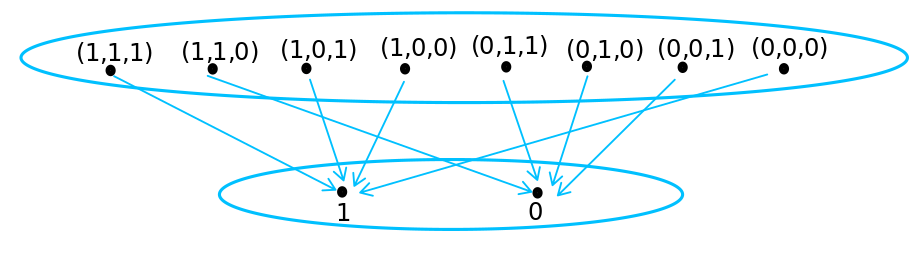
\includegraphics[scale=0.4]{../images/7.1.30.b.png}
\end{figure}
\end{proof}

\subsection{Exercise 31}
Fill in the following table to show the values of all possible two-place Boolean functions.

\begin{proof}
\begin{center}
\arrayrulecolor{cyan}
\begin{tabular}{|c|c|c|c|c|c|c|c|c|c|c|c|c|c|c|c|c|}
\hline
{\bf Input} & \(\bm{f_{1}}\) & \(\bm{f_{2}}\) & 
\(\bm{f_{3}}\) & \(\bm{f_{4}}\) & \(\bm{f_{5}}\) & 
\(\bm{f_{6}}\) & \(\bm{f_{7}}\) & \(\bm{f_{8}}\) & 
\(\bm{f_{9}}\) & \(\bm{f_{10}}\) & \(\bm{f_{11}}\) & 
\(\bm{f_{12}}\) & \(\bm{f_{13}}\) & \(\bm{f_{14}}\) & 
\(\bm{f_{15}}\) & \(\bm{f_{16}}\) \\
\hline
1 1 &0&0&0&0&0&0&0&0&1&1&1&1&1&1&1&1 \\
\hline
1 0 &0&0&0&0&1&1&1&1&0&0&0&0&1&1&1&1 \\
\hline
0 1 &0&0&1&1&0&0&1&1&0&0&1&1&0&0&1&1 \\
\hline
0 0 &0&1&0&1&0&1&0&1&0&1&0&1&0&1&0&1 \\
\hline
\end{tabular}
\arrayrulecolor{black} % change it back!
\end{center}
\end{proof}

\subsection{Exercise 32}
Consider the three-place Boolean function $f$ defined by the following rule: For each triple \((x_1, x_2, x_3)\) of
0’s and 1’s,
\[
f(x_1, x_2, x_3) = (4x_1 + 3x_2 + 2x_3) \mod 2.
\]
\subsubsection{(a)}
Find $f(1, 1, 1)$ and $f(0, 0, 1)$.

\begin{proof}
\(f(1, 1, 1) = (4 \cdot 1 + 3 \cdot 1 + 2 \cdot 1) \mod 2 = 9 \mod 2 = 1\)

\(f(0, 0, 1) = (4 \cdot 0 + 3 \cdot 0 + 2 \cdot 1) \mod 2 = 2 \mod 2 = 0\)
\end{proof}

\subsubsection{(b)}
Describe $f$ using an input/output table.

\begin{proof}
\begin{center}
\arrayrulecolor{cyan}
\begin{tabular}{|ccc|c|}
\hline
\multicolumn{3}{|c|}{\cy Input} & {\cy Output} \\
\hline
$x_1$ & $x_2$ & $x_3$ & $f(x_1, x_2, x_3)$ \\
\hline
1 & 1 & 1 & 1 \\
\hline
1 & 1 & 0 & 1 \\
\hline
1 & 0 & 1 & 0 \\
\hline
1 & 0 & 0 & 0 \\
\hline
0 & 1 & 1 & 1 \\
\hline
0 & 1 & 0 & 1 \\
\hline
0 & 0 & 1 & 0 \\
\hline
0 & 0 & 0 & 0 \\
\hline
\end{tabular}
\arrayrulecolor{black}
\end{center}
\end{proof}

\subsection{Exercise 33}
Student $A$ tries to define a function \(g: \Q \to \Z\) by
the rule
\[
g \left(\frac{m}{n}\right) = m-n \text{ for all integers } m \text{ and } n \text{ with } n \neq 0.
\]
Student $B$ claims that $g$ is not well defined. Justify student $B$'s claim.

\begin{proof}
If $g$ were well defined, then \(g(1/2) = g(2/4)\) because \(1/2 = 2/4\). However, \(g(1/2) = 1 - 2 = -1\) and 
\(g(2/4) = 2 - 4 = -2\). Since \(-1 \neq -2, g(1/2) \neq g(2/4)\). Thus $g$ is not well defined.
\end{proof}

\subsection{Exercise 34}
Student $C$ tries to define a function \(h: \Q \to \Q\) by
the rule
\[
h \left(\frac{m}{n}\right) = \frac{m^2}{n} \text{ for all integers } m \text{ and } n \text{ with } n \neq 0.
\]
Student $D$ claims that $h$ is not well defined. Justify student $D$'s claim.

\begin{proof}
\[
h(2) = h\left(\frac{4}{2}\right) = \frac{4^2}{2} = 8 \neq 4 = \frac{2^2}{1} = h\left(\frac{2}{1}\right) = h(2).
\]
\end{proof}

\subsection{Exercise 35}
Let \(U = \{1, 2, 3, 4\}\). Student $A$ tries to define a function \(R: U \to \Z\) as follows: For each \(x \in U\), 
\(R(x)\) is the integer $y$ so that \((xy) \mod 5 = 1\). Student $B$ claims that $R$ is not well defined. Who is 
right: student $A$ or student $B$? Justify your answer.

\begin{proof}
Student $B$ is correct. If $R$ were well defined, then $R(3)$ would have a uniquely determined value. However, on 
the one hand, \(R(3) = 2\) because \((3 \cdot 2) \mod 5 = 1\), and, on the other hand, \(R(3) = 7\) because 
\((3 \cdot 7) \mod 5 = 1\). Hence \(R(3)\) does not have a uniquely determined value, and so $R$ is not well defined.
\end{proof}

\subsection{Exercise 36}
Let \(V = \{1, 2, 3\}\). Student $C$ tries to define a function \(S: V \to V\) as follows: For each \(x \in V\), 
\(S(x)\) is the integer $y$ in $V$ so that \((xy) \mod 4 = 1\). Student $D$ claims that $S$ is not well defined. Who 
is right: student $C$ or student $D$? Justify your answer.

\begin{proof}
Student $D$ is right, because $S(2)$ is not defined. \(2 \cdot 1 \mod 4 = 2, 2 \cdot 2 \mod 4 = 0\), and
\(2 \cdot 3 \mod 4 = 2\). So when $x = 2$ there is no $y$ in $V$ such that \(xy \mod 4 = 1\).
\end{proof}

\subsection{Exercise 37}
On certain computers the integer data type goes from -2,147,483,648 to 2,147,483,647. Let $S$ be the set of 
all integers from -2,147,483,648 through 2,147,483,647. Try to define a function \(f: S \to S\) by the rule 
\(f(n) = n^2\) for each $n$ in $S$. Is $f$ well defined? Explain.

\begin{proof}
No, \(2,147,483,647 = 2^{31} - 1\) so for values of $n$ greater than, say, $2^{16}$, \(f(n) = n^2\) will be greater 
than $2^{32}$ which falls outside of $S$. 

Computers handle this by using 2's complement and looping the overshoot around back to \(-2^{31}\) and onward toward 
the positive values again. Here is an example from Scala:

\begin{minted}{scala}
$ scala
// Welcome to Scala 3.3.0 (17.0.7, Java OpenJDK 64-Bit Server VM). 
// Type in expressions for evaluation. Or try :help.
scala> def f(n: Int): Int = n*n
def f(n: Int): Int                                    
scala> f(2147483647)
val res0: Int = 1
scala> 
\end{minted}
\end{proof}

\subsection{Exercise 38}
Let \(X = \{a,b,c\}\) and \(Y = \{r,s,t,u,v,w\}\). Define \(f: X \to Y\) as follows: \(f(a) = b, f(b) = v, f(c) = t\).

\subsubsection{(a)}
Draw an arrow diagram for $f$.

\begin{proof}
\begin{figure}[ht!]
\centering
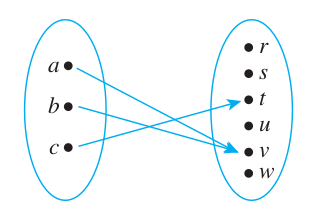
\includegraphics[scale=0.5]{../images/7.1.38.a.png}
\end{figure}
\end{proof}

\subsubsection{(b)}
Let \(A = \{a, b\}, C = \{t\}, D = \{u, v\}, E = \{r, s\}\). 

Find \(f(A), f(X), f^{-1}(C), f^{-1}(D), f^{-1}(E), f^{-1}(Y)\).

\begin{proof}
\(f(A) = \{v\}, f(X) = \{t, v\}, f^{-1}(C) = \{c\}, f^{-1}(D) = \{a, b\}, f^{-1}(E) = \es\), 

\(f^{-1}(Y) = \{a,b,c\}\)
\end{proof}

\subsection{Exercise 39}
Let \(X = \{1, 2, 3, 4\}\) and \(Y = \{a, b, c, d, e\}\). Define \(g: X \to Y\) as follows: 
\(g(1) = a, g(2) = a, g(3) = a, g(4) = d\).

\subsubsection{(a)}
Draw an arrow diagram for $g$.

\begin{proof}
\begin{figure}[ht!]
\centering
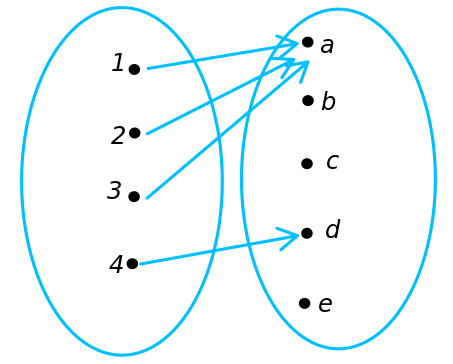
\includegraphics[scale=0.3]{../images/7.1.39.a.png}
\end{figure}
\end{proof}

\subsubsection{(b)}
Let \(A = \{2, 3\}, C = \{a\}\), and \(D = \{b, c\}\). Find \(g(A), g(X), g^{-1}(C), g^{-1}(D)\), and \(g^{-1}(Y)\).

\begin{proof}
\(g(A) = \{a\}, g(X) = \{a, d\}, g^{-1}(C) = \{1, 2, 3\}, g^{-1}(D) = \es, g^{-1}(Y) = \{1, 2, 3, 4\}\).
\end{proof}

\subsection{Exercise 40}
Let $X$ and $Y$ be sets, let $A$ and $B$ be any subsets of $X$, and let $F$ be a function from $X$ to $Y$. Fill in the 
blanks in the following proof that \(F(A) \cup F (B) \subseteq F(A \cup B)\).

{\bf Proof:} Let $y$ be any element in \(F(A) \cup F(B)\). {\it [We must show that $y$ is in \(F(A \cup B)\).]} By 
definition of union, {\cy (i) \fbl.} 

{\bf Case 1, \(\bm{y \in F(A)}\):} In this case, by definition of $F(A)$, \(y = F(x)\) for {\cy (ii) \fbl} 
\(x \in A\). Since \(A \subseteq A \cup B\), it follows from the definition of union that \(x \in\) {\cy (iii) 
\fbl.} Hence, \(y = F(x)\) for some \(x \in A \cup B\), and thus, by definition of \(F(A \cup B), y \in\) {\cy (iv) \fbl.}

{\bf Case 2, \(\bm{y \in F(B)}\):} In this case, by definition of $F(B)$, {\cy (v) \fbl} for some $x \in B$. 
Since \(B \subseteq A \cup B\) it follows from the definition of union that {\cy (vi) \fbl.} 
Thus \(y \in F(A \cup B)\).

Therefore, regardless of whether \(y \in F(A)\) or \(y \in F(B)\), we have that \(y \in F(A \cup B)\) {\it [as was to be shown].}

\begin{proof}
(i) \(y \in F(A)\) or \(y \in F(B)\) (ii) some (iii) \(A \cup B\) (iv) \(F(A \cup B)\) (v) \(y = F(x)\) (vi) \(x \in A \cup B\)
\end{proof}

{\bf \cy In $41-49$ let $X$ and $Y$ be sets, let $A$ and $B$ be any subsets of $X$, and let $C$ and $D$ be any 
subsets of $Y$. Determine which of the properties are true for every function $F$ from $X$ to $Y$ and which are false 
for at least one function $F$ from $X$ to $Y$. Justify your answers.}

\subsection{Exercise 41}
If \(A \subseteq B\) then \(F(A) \subseteq F(B)\).

\begin{proof}
Let $F$ be a function from $X$ to $Y$, and suppose \(A \subseteq X, B \subseteq X\), and \(A \subseteq B\). 
Let \(y \in F(A)\). {\it [We must show that \(y \in F(B)\).]} By definition of image of a set, \(y = F(x)\) for 
some \(x \in A\). Thus since \(A \subseteq B, x \in B\), and so \(y = F(x)\) for some \(x \in B\). 
Hence \(y \in F(B)\) {\it [as was to be shown].}
\end{proof}

\subsection{Exercise 42}
\(F(A \cap B) \subseteq F(A) \cap F(B)\)

\begin{proof}
1. Assume \(y \in F(A \cap B)\). {\it [We want to show \(y \in F(A) \cap F(B)\).]} 

2. By 1 and definition of \(F(A \cap B)\), \(y = F(x)\) for some \(x \in A \cap B\).

3. By 2 and definition of intersection, \(x \in A\) and \(x \in B\).

4. By 3 and definition of $F(A)$ and $F(B)$, \(y = F(x)\) is in $F(A)$ and in $F(B)$.

5. By 4 and definition of intersection, \(y \in F(A) \cap F(B)\).

6. By 1, 5 and definition of subset, \(F(A \cap B) \subseteq F(A) \cap F(B)\).
\end{proof}

\subsection{Exercise 43}
\(F(A) \cap F(B) \subseteq F(A \cap B)\)

\begin{proof}
\begin{figure}[ht!]
\centering
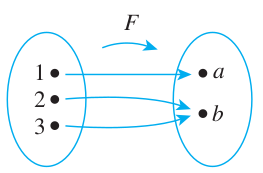
\includegraphics[scale=0.5]{../images/7.1.43.png}
\end{figure}
\underline{Counterexample:} Let \(X = \{1, 2, 3\}\), let \(Y = \{a, b\}\), and define a function \(F: X \to Y\) 
by the arrow diagram shown above.

Let \(A = \{1, 2\}\) and \(B = \{1, 3\}\). Then \(F(A) = \{a, b\} = F(B)\), and so \(F(A) \cap F(B) = \{a, b\}\). But 
\(F(A \cap B) = F(\{1\}) = \{a\} \neq \{a, b\}\). And so \(F(A) \cap F(B) \nsubseteq F(A \cap B)\). (This is just one 
of many possible counterexamples.)
\end{proof}

\subsection{Exercise 44}
For all subsets $A$ and $B$ of $X$, \(F(A - B) = F(A) - F(B)\).

\begin{proof}
\underline{Counterexample:} Let \(X = \{1, 2\}, Y = \{a\}, A = \{1\}, B = \{2\}\), define \(F: X \to Y\) by 
\(F(1) = F(2) = a\). Then \(A - B = \{1\}, F(A) = \{a\}, F(B)=\{a\}\). So \(F(A-B) = \{a\} \neq \es = F(A) - F(B)\).
\end{proof}

\subsection{Exercise 45}
For all subsets $C$ and $D$ of $Y$, if \(C \subseteq D\) then \(F^{-1}(C) \subseteq F^{-1}(D)\).

\begin{proof}
Let $F$ be a function from a set $X$ to a set $Y$, and suppose \(C \subseteq Y, D \subseteq Y\), and 
\(C \subseteq D\). {\it [We must show that \(F^{-1}(C) \subseteq F^{-1}(D)\).]} Suppose \(x \in F^{-1}(C)\). Then 
\(F(x) \in C\). Since \(C \subseteq D, F(x) \in D\) also. Hence, by definition of inverse image, \(x \in F^{-1}(D)\). 
{\it [So \(F^{-1}(C) \subseteq F^{-1}(D)\).]}
\end{proof}

\subsection{Exercise 46}
For all subsets $C$ and $D$ of $Y$, \(F^{-1}(C \cup D) = F^{-1}(C) \cup F^{-1}(D)\).

\begin{proof}
1. Assume \(x \in F^{-1}(C \cup D)\) and let $y = F(x)$. {\it [Want to show \(x \in F^{-1}(C) \cup F^{-1}(D)\).]}

2. By 1 and definition of \(F^{-1}(C \cup D)\), \(y \in C \cup D\).

3. By 2 and definition of union, \(y \in C\) or \(y \in D\).

4. {\bf Case 1 (\(\bm{y \in C}\)):} By definition of \(F^{-1}(C)\), \(x \in F^{-1}(C)\). 

By definition of union, \(x \in F^{-1}(C) \cup F^{-1}(D)\).

5. {\bf Case 2 (\(\bm{y \in D}\)):} By definition of \(F^{-1}(D)\), \(x \in F^{-1}(D)\). 

By definition of union, \(x \in F^{-1}(C) \cup F^{-1}(D)\).

6. By 4 and 5, \(x \in F^{-1}(C) \cup F^{-1}(D)\).

7. By 1, 6 and definition of subset, \(F^{-1}(C \cup D) \subseteq F^{-1}(C) \cup F^{-1}(D)\).

The proof of the reverse direction \(F^{-1}(C) \cup F^{-1}(D) \subseteq F^{-1}(C \cup D)\) is similar.
\end{proof}

\subsection{Exercise 47}
For all subsets $C$ and $D$ of $Y$, \(F^{-1}(C \cap D) = F^{-1}(C) \cap F^{-1}(D)\).

\begin{proof}
True, the proof is extremely similar to exercise 46.
\end{proof}

\subsection{Exercise 48}
For all subsets $C$ and $D$ of $Y$, \(F^{-1}(C-D) = F^{-1}(C) - F^{-1}(D)\).

\begin{proof}
1. Assume \(x \in F^{-1}(C-D)\) and let $y = F(x)$. {\it [Want to show \(x \in F^{-1}(C) - F^{-1}(D)\).]}

2. By 1 and definition of \(F^{-1}(C-D), y \in C-D\).

3. By 2 and definition of difference, \(y \in C\) and \(y \notin D\).

4. By 3 and definition of \(F^{-1}(C)\), \(x \in F^{-1}(C)\). Similarly, since $y = F(x)$ and $y \notin D$, 
\(x \notin F^{-1}(D)\).

5. By 4 and definition of difference, \(x \in F^{-1}(C) - F^{-1}(D)\).

6. By 1, 5 and definition of subset, \(F^{-1}(C-D) \subseteq F^{-1}(C) - F^{-1}(D)\).

{\it Now the reverse part:}

7. Assume \(x \in F^{-1}(C) - F^{-1}(D)\) and let $y = F(x)$. {\it [Want to show \(x \in F^{-1}(C-D)\).]}

8. By 7 and definition of difference, \(x \in F^{-1}(C)\) and \(x \notin F^{-1}(D)\).

9. By 8 and definition of \(F^{-1}(C), y \in C\). Similarly \(y \notin D\).

10. By 9 and definition of difference \(y \in C-D\).

11. Since $y = F(x)$, by 10 and definition of \(F^{-1}(C-D)\), \(x \in F^{-1}(C-D)\).

12. By 7, 11 and definition of subset, \(F^{-1}(C) - F^{-1}(D) \subseteq F^{-1}(C-D)\).

{\it Conclusion:}

13. By 6, 12 and definition of set equality \(F^{-1}(C) - F^{-1}(D) = F^{-1}(C-D)\).
\end{proof}

\subsection{Exercise 49}
\(F(F^{-1}(C)) \subseteq C\).

\begin{proof}
1. Assume \(y \in F(F^{-1}(C))\). {\it [Want to show \(y \in C\).]}

2. By 1 and definition of \(F(F^{-1}(C))\), there exists some \(x \in F^{-1}(C)\) such that \(y = F(x)\).

3. By 2 and definition of \(F^{-1}(C)\), \(F(x) \in C\). So $y \in C$ because $y = F(x)$.

4. By 1, 3 and definition of subset, \(F(F^{-1}(C)) \subseteq C\).
\end{proof}

\subsection{Exercise 50}
Given a set $S$ and a subset $A$, the characteristic function of $A$, denoted $\chi_A$, is the function defined 
from $S$ to $\Z$ with the property that for each $u \in S$,
\[
\chi_A(u) =
\left\{
\begin{tabular}{lr}
\(1\) & if \(u \in A\) \\
\(0\) & if \(u \notin A\)
\end{tabular}
\right.
\]
Show that each of the following holds for all subsets $A$ and $B$ of $S$ and every $u \in S$.

\subsubsection{(a)}
\(\chi_{A \cap B}(u) = \chi_A(u) \cdot \chi_B(u)\)

\begin{proof}
Assume $A, B$ are any subsets of $S$ and $u$ is any element in $S$. There are 4 cases:

{\bf Case 1 (\(\bm{u \in A, u \in B}\)):} Then \(\chi_A(u) = 1 \) and \(\chi_B(u) = 1\). 

By definition of intersection \(u \in A \cap B\). Thus
\(\chi_{A \cap B}(u) = 1\) also. Since $1 = 1 \cdot 1$,
\(\chi_{A \cap B}(u) = \chi_A(u) \cdot \chi_B(u)\).

{\bf Case 2 (\(\bm{u \in A, u \notin B}\)):} Then \(\chi_A(u) = 1 \) and \(\chi_B(u) = 0\). 

By definition of intersection \(u \notin A \cap B\). Thus
\(\chi_{A \cap B}(u) = 0\) also. Since $0 = 1 \cdot 0$,
\(\chi_{A \cap B}(u) = \chi_A(u) \cdot \chi_B(u)\).

{\bf Case 3 (\(\bm{u \notin A, u \in B}\)):} Then \(\chi_A(u) = 0 \) and \(\chi_B(u) = 1\). 

By definition of intersection \(u \notin A \cap B\). Thus
\(\chi_{A \cap B}(u) = 0\) also. Since $0 = 0 \cdot 1$,
\(\chi_{A \cap B}(u) = \chi_A(u) \cdot \chi_B(u)\).

{\bf Case 4 (\(\bm{u \notin A, u \notin B}\)):} Then \(\chi_A(u) = 0 \) and \(\chi_B(u) = 0\). 

By definition of intersection \(u \notin A \cap B\). Thus
\(\chi_{A \cap B}(u) = 0\) also. Since $0 = 0 \cdot 0$,
\(\chi_{A \cap B}(u) = \chi_A(u) \cdot \chi_B(u)\).
\end{proof}

\subsubsection{(b)}
\(\chi_{A \cup B}(u) = \chi_A(u) + \chi_B(u) - \chi_A(u) \cdot \chi_B(u)\)

\begin{proof}
Assume $A, B$ are any subsets of $S$ and $u$ is any element in $S$. There are 4 cases:

{\bf Case 1 (\(\bm{u \in A, u \in B}\)):} Then \(\chi_A(u) = 1 \) and \(\chi_B(u) = 1\). 

By definition of union \(u \in A \cup B\). Thus
\(\chi_{A \cup B}(u) = 1\) also. 
Since $1 = 1 + 1 - (1 \cdot 1)$, \(\chi_{A \cup B}(u) = \chi_A(u) + \chi_B(u) - \chi_A(u) \cdot \chi_B(u)\).

{\bf Case 2 (\(\bm{u \in A, u \notin B}\)):} Then \(\chi_A(u) = 1\) and \(\chi_B(u) = 0\). 

By definition of union \(u \in A \cup B\). Thus
\(\chi_{A \cup B}(u) = 1\) also. 
Since $1 = 1 + 0 - (1 \cdot 0)$, \(\chi_{A \cup B}(u) = \chi_A(u) + \chi_B(u) - \chi_A(u) \cdot \chi_B(u)\).

{\bf Case 3 (\(\bm{u \notin A, u \in B}\)):} Then \(\chi_A(u) = 0\) and \(\chi_B(u) = 1\). 

By definition of union \(u \in A \cup B\). Thus
\(\chi_{A \cup B}(u) = 1\) also. 
Since $1 = 0 + 1 - (0 \cdot 1)$, \(\chi_{A \cup B}(u) = \chi_A(u) + \chi_B(u) - \chi_A(u) \cdot \chi_B(u)\).

{\bf Case 4 (\(\bm{u \notin A, u \notin B}\)):} Then \(\chi_A(u) = 0 \) and \(\chi_B(u) = 0\). 

By definition of union \(u \notin A \cup B\). Thus
\(\chi_{A \cup B}(u) = 0\) also. 
Since $0 = 0 + 0 - (0 \cdot 0)$, \(\chi_{A \cup B}(u) = \chi_A(u) + \chi_B(u) - \chi_A(u) \cdot \chi_B(u)\).
\end{proof}

{\bf \cy Each of exercises $51-53$ refers to the Euler phi function, denoted $\phi$, which is defined as follows: For 
each integer \(n \geq 1\), $\phi(n)$ is the number of positive integers less than or equal to $n$ that have no 
common factors with $n$ except $\pm 1$. For example, \(\phi(10) = 4\) because there are four positive integers 
less than or equal to 10 that have no common factors with 10 except $\pm 1$, namely, 1, 3, 7, and 9.}

\subsection{Exercise 51}
Find each of the following:

\subsubsection{(a)}
\(\phi(15)\)

\begin{proof}
\(\phi(15) = 8\) {\it [because $1, 2, 4, 7, 8, 11, 13$, and $14$ have no common factors with $15$ other than $\pm 1$]}
\end{proof}

\subsubsection{(b)}
\(\phi(2)\)

\begin{proof}
\(\phi(2) = 1\) {\it [because the only positive integer less than or equal to $2$ having no common factors with $2$ 
other than $\pm 1$ is $1$]}
\end{proof}

\subsubsection{(c)}
\(\phi(5)\)

\begin{proof}
\(\phi(5) = 4\) {\it [because $1, 2, 3$, and $4$ have no common factors with $5$ other than $\pm 1$]}
\end{proof}

\subsubsection{(d)}
\(\phi(12)\)

\begin{proof}
\(\phi(12) = 4\) (1, 5, 7, 11)
\end{proof}

\subsubsection{(e)}
\(\phi(11)\)

\begin{proof}
\(\phi(11) = 10\) (1, 2, 3, 4, 5, 6, 7, 8, 9, 10)
\end{proof}

\subsubsection{(f)}
\(\phi(1)\)

\begin{proof}
\(\phi(1) = 1\)
\end{proof}

\subsection{Exercise 52}
Prove that if $p$ is a prime number and $n$ is an integer with \(n \geq 1\), then \(\phi(p^n) = p^n - p^{n-1}\).

\begin{proof}
Let $p$ be any prime number and $n$ any integer with \(n \geq 1\). There are \(p^{n-1}\) positive integers less than 
or equal to \(p^n\) that have a common factor other than $\pm 1$ with \(p^n\), namely, \(p, 2p, 3p, \ldots, 
(p^{n-1})p\). Hence, there are \(p^n - p^{n-1}\) positive integers less than or equal to \(p^n\) that do not have a 
common factor with \(p^n\) except for $\pm 1$.
\end{proof}

\subsection{Exercise 53}
Prove that there are infinitely many integers $n$ for which \(\phi(n)\) is a perfect square.

\begin{proof}
By exercise 52, for any integer $n$ with \(n \geq 1, \phi(2^n) = 2^n - 2^{n-1} = 2^{n-1}\).

So, for all integers $k$ with $k \geq 1$, we have that \(\phi(2^{2k+1}) = 2^{2k} = (2^k)^2\) is a perfect square.
\end{proof}

\section{Exercise Set 7.2}

\subsection{Exercise 1}

\begin{proof}

\end{proof}

\subsection{Exercise 2}

\begin{proof}

\end{proof}

\subsection{Exercise 3}

\begin{proof}

\end{proof}

\subsection{Exercise 4}

\begin{proof}

\end{proof}

\subsection{Exercise 5}

\begin{proof}

\end{proof}

\subsection{Exercise 6}

\begin{proof}

\end{proof}

\subsection{Exercise 7}

\begin{proof}

\end{proof}

\subsection{Exercise 8}

\begin{proof}

\end{proof}

\subsection{Exercise 9}

\begin{proof}

\end{proof}

\subsection{Exercise 10}

\begin{proof}

\end{proof}

\subsection{Exercise 11}

\begin{proof}

\end{proof}

\subsection{Exercise 12}

\begin{proof}

\end{proof}

\subsection{Exercise 13}

\begin{proof}

\end{proof}

\subsection{Exercise 14}

\begin{proof}

\end{proof}

\subsection{Exercise 15}

\begin{proof}

\end{proof}

\subsection{Exercise 16}

\begin{proof}

\end{proof}

\subsection{Exercise 17}

\begin{proof}

\end{proof}

\subsection{Exercise 18}

\begin{proof}

\end{proof}

\subsection{Exercise 19}

\begin{proof}

\end{proof}

\subsection{Exercise 20}

\begin{proof}

\end{proof}

\subsection{Exercise 21}

\begin{proof}

\end{proof}

\subsection{Exercise 22}

\begin{proof}

\end{proof}

\subsection{Exercise 23}

\begin{proof}

\end{proof}

\subsection{Exercise 24}

\begin{proof}

\end{proof}

\subsection{Exercise 25}

\begin{proof}

\end{proof}

\subsection{Exercise 26}

\begin{proof}

\end{proof}

\subsection{Exercise 27}

\begin{proof}

\end{proof}

\subsection{Exercise 28}

\begin{proof}

\end{proof}

\subsection{Exercise 29}

\begin{proof}

\end{proof}

\subsection{Exercise 30}

\begin{proof}

\end{proof}

\subsection{Exercise 31}

\begin{proof}

\end{proof}

\subsection{Exercise 32}

\begin{proof}

\end{proof}

\subsection{Exercise 33}

\begin{proof}

\end{proof}

\subsection{Exercise 34}

\begin{proof}

\end{proof}

\subsection{Exercise 35}

\begin{proof}

\end{proof}

\subsection{Exercise 36}

\begin{proof}

\end{proof}

\subsection{Exercise 37}

\begin{proof}

\end{proof}

\subsection{Exercise 38}

\begin{proof}

\end{proof}

\subsection{Exercise 39}

\begin{proof}

\end{proof}

\subsection{Exercise 40}

\begin{proof}

\end{proof}

\subsection{Exercise 41}

\begin{proof}

\end{proof}

\subsection{Exercise 42}

\begin{proof}

\end{proof}

\subsection{Exercise 43}

\begin{proof}

\end{proof}

\subsection{Exercise 44}

\begin{proof}

\end{proof}

\subsection{Exercise 45}

\begin{proof}

\end{proof}

\subsection{Exercise 46}

\begin{proof}

\end{proof}

\subsection{Exercise 47}

\begin{proof}

\end{proof}

\subsection{Exercise 48}

\begin{proof}

\end{proof}

\subsection{Exercise 49}

\begin{proof}

\end{proof}

\subsection{Exercise 50}

\begin{proof}

\end{proof}

\subsection{Exercise 51}

\begin{proof}

\end{proof}

\subsection{Exercise 52}

\begin{proof}

\end{proof}

\subsection{Exercise 53}

\begin{proof}

\end{proof}

\subsection{Exercise 54}

\begin{proof}

\end{proof}

\subsection{Exercise 55}

\begin{proof}

\end{proof}

\subsection{Exercise 56}

\begin{proof}

\end{proof}

\subsection{Exercise 57}

\begin{proof}

\end{proof}

\subsection{Exercise 58}

\begin{proof}

\end{proof}

\end{document}

\section{Exercise Set 7.3}

\subsection{Exercise 1}

\begin{proof}

\end{proof}

\subsection{Exercise 2}

\begin{proof}

\end{proof}

\subsection{Exercise 3}

\begin{proof}

\end{proof}

\subsection{Exercise 4}

\begin{proof}

\end{proof}

\subsection{Exercise 5}

\begin{proof}

\end{proof}

\subsection{Exercise 6}

\begin{proof}

\end{proof}

\subsection{Exercise 7}

\begin{proof}

\end{proof}

\subsection{Exercise 8}

\begin{proof}

\end{proof}

\subsection{Exercise 9}

\begin{proof}

\end{proof}

\subsection{Exercise 10}

\begin{proof}

\end{proof}

\subsection{Exercise 11}

\begin{proof}

\end{proof}

\subsection{Exercise 12}

\begin{proof}

\end{proof}

\subsection{Exercise 13}

\begin{proof}

\end{proof}

\subsection{Exercise 14}

\begin{proof}

\end{proof}

\subsection{Exercise 15}

\begin{proof}

\end{proof}

\subsection{Exercise 16}

\begin{proof}

\end{proof}

\subsection{Exercise 17}

\begin{proof}

\end{proof}

\subsection{Exercise 18}

\begin{proof}

\end{proof}

\subsection{Exercise 19}

\begin{proof}

\end{proof}

\subsection{Exercise 20}

\begin{proof}

\end{proof}

\subsection{Exercise 21}

\begin{proof}

\end{proof}

\subsection{Exercise 22}

\begin{proof}

\end{proof}

\subsection{Exercise 23}

\begin{proof}

\end{proof}

\subsection{Exercise 24}

\begin{proof}

\end{proof}

\subsection{Exercise 25}

\begin{proof}

\end{proof}

\subsection{Exercise 26}

\begin{proof}

\end{proof}

\subsection{Exercise 27}

\begin{proof}

\end{proof}

\subsection{Exercise 28}

\begin{proof}

\end{proof}

\subsection{Exercise 29}

\begin{proof}

\end{proof}

\subsection{Exercise 30}

\begin{proof}

\end{proof}

\section{Exercise Set 7.4}

\subsection{Exercise 1}

\begin{proof}

\end{proof}

\subsection{Exercise 2}

\begin{proof}

\end{proof}

\subsection{Exercise 3}

\begin{proof}

\end{proof}

\subsection{Exercise 4}

\begin{proof}

\end{proof}

\subsection{Exercise 5}

\begin{proof}

\end{proof}

\subsection{Exercise 6}

\begin{proof}

\end{proof}

\subsection{Exercise 7}

\begin{proof}

\end{proof}

\subsection{Exercise 8}

\begin{proof}

\end{proof}

\subsection{Exercise 9}

\begin{proof}

\end{proof}

\subsection{Exercise 10}

\begin{proof}

\end{proof}

\subsection{Exercise 11}

\begin{proof}

\end{proof}

\subsection{Exercise 12}

\begin{proof}

\end{proof}

\subsection{Exercise 13}

\begin{proof}

\end{proof}

\subsection{Exercise 14}

\begin{proof}

\end{proof}

\subsection{Exercise 15}

\begin{proof}

\end{proof}

\subsection{Exercise 16}

\begin{proof}

\end{proof}

\subsection{Exercise 17}

\begin{proof}

\end{proof}

\subsection{Exercise 18}

\begin{proof}

\end{proof}

\subsection{Exercise 19}

\begin{proof}

\end{proof}

\subsection{Exercise 20}

\begin{proof}

\end{proof}

\subsection{Exercise 21}

\begin{proof}

\end{proof}

\subsection{Exercise 22}

\begin{proof}

\end{proof}

\subsection{Exercise 23}

\begin{proof}

\end{proof}

\subsection{Exercise 24}

\begin{proof}

\end{proof}

\subsection{Exercise 25}

\begin{proof}

\end{proof}

\subsection{Exercise 26}

\begin{proof}

\end{proof}

\subsection{Exercise 27}

\begin{proof}

\end{proof}

\subsection{Exercise 28}

\begin{proof}

\end{proof}

\subsection{Exercise 29}

\begin{proof}

\end{proof}

\subsection{Exercise 30}

\begin{proof}

\end{proof}

\subsection{Exercise 31}

\begin{proof}

\end{proof}

\subsection{Exercise 32}

\begin{proof}

\end{proof}

\subsection{Exercise 33}

\begin{proof}

\end{proof}

\subsection{Exercise 34}

\begin{proof}

\end{proof}

\subsection{Exercise 35}

\begin{proof}

\end{proof}

\subsection{Exercise 36}

\begin{proof}

\end{proof}

\subsection{Exercise 37}

\begin{proof}

\end{proof}

\subsection{Exercise 38}

\begin{proof}

\end{proof}

\end{document}
